\section{Traditional control model}

Anthony's Pyramid is a well-established framework for understanding how organizations manage control across different levels. It breaks down the process into three distinct types of control
\begin{enumerate}
    \item \textit{Strategic control}: setting and monitoring the organization's overall business objectives.
    \item \textit{Management control}: managing financial resources effectively. 
    \item \textit{Operational control}: ensures daily operating activities are carried out efficiently and effectively.
\end{enumerate}
\begin{figure}[H]
    \centering
    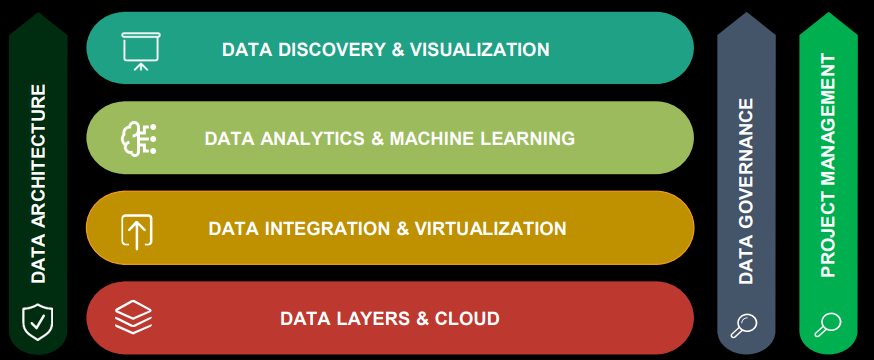
\includegraphics[width=0.5\linewidth]{images/bis3.png}
    \caption{Anthony's pyramid}
\end{figure}